%%========================================
%% Commands: pdflatex tese
%%           bibtex tese
%%           makeindex tese (only if creating an index)
%%           pdflatex tese
%% Alternative
%%          latexmk -pdf tese.tex
%%========================================

\documentclass[11pt,a4paper,twoside,openright]{report}

%% For iso-8859-1 (latin1), comment next line and uncomment the second line
\usepackage[utf8]{inputenc}
%\usepackage[latin1]{inputenc}
\usepackage{listings}
%% English version

%% MIEEC options
\usepackage[mieec]{feupteses}
%\usepackage[mieec,juri]{feupteses}
%\usepackage[mieec,final]{feupteses}


%% Additional options for feupteses.sty:
%% - onpaper: links are not shown (for paper versions)
%% - backrefs: include back references from bibliography to citation  place

%% Uncomment to create an index (at the end of the document)
%\makeindex

%% Path to the figures directory
%% TIP: use folder ``figures'' to keep all your figures
\graphicspath{{figures/}}

%%----------------------------------------
%% TIP: if you want to define more macros, use an external file to keep them
%some macro definitions

% format
%\newcommand{\class}[1]{{\normalfont\slshape #1\/}}

% entities
\newcommand{\Feup}{Faculdade de Engenharia da Universidade do Porto}

\newcommand{\svg}{\class{SVG}}
\newcommand{\scada}{\class{SCADA}}
\newcommand{\scadadms}{\class{SCADA/DMS}}

\addto\extrasenglish{
	\renewcommand{\chapterautorefname}{Chapter}
}

%%----------------------------------------

%%========================================
%% Start of document
%%========================================
\begin{document}

%%----------------------------------------
%% Information about the work
%%----------------------------------------
\title{Real-Time Ethernet Networks: a practical approach to cycle time influence in control applications}
\author{Sim\~{a}o Paulo Marques de Amorim}

%% Uncomment next line for date of submission
%\thesisdate{July 31, 2008}

%% Comment next line copyright text if not used
\copyrightnotice{Sim\~{a}o Paulo Marques de Amorim, 2021}

\supervisor{Supervisor}{Paulo Jos\'{e} Lopes Machado Portugal}

%% Uncomment next line if necessary
%\supervisor{Second Supervisor}{Name of the Supervisor}

%% Uncomment committee stuff in the final version if used
%\committeetext{Approved by \ldots:}
%\committeemember{President}{Name of the President}
%\committeemember{Referee}{Name of the Referee}
%\committeemember{Referee}{Name of the Referee}
%\signature

%% Specify cover logo (in folder ``figures'')
\logo{uporto-feup.pdf}

%% Uncomment next line for additional text  below the author's name (front page)

%%----------------------------------------
%% Preliminary materials
%%----------------------------------------

% remove unnecessary \include{} commands
\begin{Prolog}
  \chapter*{Abstract}
%\addcontentsline{toc}{chapter}{Abstract}
We live in an increasingly digital and computerised world where there is a constant need for interconnection between everything and everyone.
Ethernet networks quickly became the communication standard in office and home environments, but their adoption in the industrial environment has been much slower.
This reduced speed of adoption is mainly due to the non-deterministic communication that Ethernet network provides, which does not make it a viable option for automation and robotics systems that require predictable and deterministic communications.
Modern automation and robotic systems do not escape the accelerated need for constant interconnection and, therefore, it is necessary to adapt them, taking into account their real-time requirements.
There are several well-established real-time Ethernet network solutions on the market, but we find the same gap on all of them: the scarcity of educational and demonstration equipment.

This document aims at presenting a solution for this gap, describing a distributed control system developed with education in mind.
The presented system focuses on the variable that mostly contributes to the deterministic characteristic of real-time Ethernet networks: the network cycle time.
The main objective is to develop a conceptual distributed control system capable of producing experimental data that demonstrates the impact that the communication network's cycle time has on control applications.
The proposed system will base itself on the implementation of a slave device for the EtherCAT network, implemented on a Raspberry Pi platform, and on the description of a possible implementation of a master device for the same network.
The implementation of the master device will purposely not be specified in detail to encourage greater involvement from the users of this system in implementing their own educational or demonstration system.

The document will begin with a presentation of the context in which this work was developed, followed by the motivation that led to the beginning of the project and a presentation of the objectives that we propose to achieve.
The state-of-the-art will consist of a presentation of real-time Ethernet networks in a generic way and an in-depth presentation of the working principle and characteristics of the EtherCAT network.
The presentation of generic real-time Ethernet networks will describe the existing categories and different approaches to the problem of non-deterministic communication in Ethernet networks.
The presentation and description of the architecture of the proposed distributed control system will follow.
Next, an explanation on how the implementation of the slave device was planned and executed, both in terms of hardware and software.
Finally, experimental results will also be presented.
These prove that the developed concept is valid and fulfils the intended characteristics.


\chapter*{Resumo}
%\addcontentsline{toc}{chapter}{Resumo}
Vivemos num mundo cada vez mais digital e informatizado onde existe uma constante necessidade de interligação entre tudo e todos.
As redes Ethernet rápidamente se tornaram no stardard da comunicação em ambientes empresariais e domésticos, mas a sua adoção no ambiente industrial tem sido bastante mais lenta.
Esta reduzida velocidade de adoção deve-se principalmente à comunicação não-determinística que a rede Ethernet proporciona, o que não a torna uma opção viável para sistemas de automação e robótica que necessitão de comunicações previsíveis e determinísticas.
Os automatismos e sistemas robóticos modernos não escapam à acelerada necessidade de constante interligação e, por isso, é necessário adaptá-los tendo em consideração os seu requisitos de tempo-real.
Existem no mercado várias soluções de redes Ethernet de comunicação de tempo real, já bem estabelecidas, mas em todas se encontra a mesma lacuna: a escassez de equipamento educativo e de demostração das mesmas.

O presente documento pretende apresentar uma solução para tal lacuna, descrevendo um sistema baseado em controlo distribuido desenvolvido a pensar na educação.
O sistema apresentado foca-se na variável com maior impacto na característica determinística das redes de Ethernet de tempo-real: o tempo de ciclo da rede.
O objectivo principal é desenvolver um conceito de um sistema de controlo distribuído capaz de produzir dados experimentais que demonstrem o impacto que o tempo de ciclo da rede de comunicação tem em aplicações de controlo.
O sistema proposto será baseado na implementação de um dispositivo escravo para a rede EtherCAT, implementado numa plataforma Raspberry Pi e na descrição de uma possível implementação de um dispositivo mestre para a mesma rede.
A implementação do dispositivo mestre será propositadamente deixada em aberto para incitar um maior envolvimento dos utilizadores deste sistema na implementação do seu próprio sistema educacional ou de demonstração.

O documento iniciará com uma apresentação do contexto em que este trabalho foi desenvolvido, seguido da motivação que levou à realização do projeto e da apresentação dos objetivos que propomos cumprir.
A revisão bibliográfica consistirá na apresentação de redes Ethernet de tempo-real de uma forma genérica e na apresentação aprofundada do modo de funcionamento e características da rede EtherCAT.
A apresentação de redes Ethernet de tempo-real genérica irá descrever as várias categorias existentes e as diferentes abordagens ao problema da falta de determinismo na comunicação Ethernet.
Seguir-se-á a apresentaçao e descrição da arquitetura do sistema de controlo distribuído proposto.
Seguidamente será explicado como foi planeada e executada a implementação do dispositivo escravo, tanto em termos de hardware como software.
Finalmente também irão ser apresentados resultados experimentais que provam que o conceito desenvolvido é válido e cumpre com as características pretendidas.

 % the abstract
  \chapter*{Acknowledgements}
%\addcontentsline{toc}{chapter}{Agradecimentos}
I want to thank professor Paulo Portugal for his continuous availability  to provide me with the best and most informed feedback possible, during all stages of the project.
Even though getting feedback has not always been easy due to the full-remote work conditions that the CODIV-19 pandemic imposed, professor Paulo Portugal made sure that all interactions were used to the fullest of what was possible, every single time.

\bigskip
I would also like to thank my family for putting up with my working habits and routines while we were all working from home.
Sometimes it wasn't easy to reconcile work and personal life, but these were definitely times where everyone had to adapt to a new reality.
As such, I'm thankful for being able to  have my own time management and working habits, but I'm also thankful that my family advised me from overworking at certain times.

\bigskip
I want to dedicate this work to my good friend Ania who helped me get through some rough times on my personal life.
Sometimes life throws a curve ball at us and suddenly nothing seems to be going the right way.
But, eventually, things become easier to overcome, especially when one has a friend that motivates us and pushes us to do our best, no matter the circumstances.

\vspace{10mm}
\flushleft{Sim\~{a}o Amorim}
  % the acknowledgments
  \cleardoublepage
\thispagestyle{plain}

\vspace*{8cm}

\begin{flushright}
%   \textsl{``You should be glad that bridge fell down. \\
%           I was planning to build thirteen more to that same design''} \\
%\vspace*{1.5cm}
%           Isambard Kingdom Brunel
	\textsl{``Tell me and I forget. Teach me and I remember. Involve me and I learn.''}\\
	\vspace*{1.5cm}
	Benjamin Franklin
\end{flushright}
    % initial quotation if desired
  \cleardoublepage
  \pdfbookmark[0]{Table of Contents}{contents}
  \tableofcontents
  \cleardoublepage
  \pdfbookmark[0]{List of Figures}{figures}
  \listoffigures
  \cleardoublepage
  \pdfbookmark[0]{List of Tables}{tables}
  \listoftables
  \chapter*{Abreviaturas e Símbolos}
%\addcontentsline{toc}{chapter}{Abbreviations}
\chaptermark{ABREVIATURAS E SÍMBOLOS}

\begin{flushleft}
\begin{tabular}{l p{0.8\linewidth}}
ADT      & Abstract Data Type\\
ANDF     & Architecture-Neutral Distribution Format\\
API      & Application Programming Interface\\
CAD      & Computer-Aided Design\\
CASE     & Computer-Aided Software Engineering\\
CORBA    & Common Object Request Broker Architecture\\
UNCOL    & UNiversal COmpiler-oriented Language\\
Loren    & Lorem ipsum dolor sit amet, consectetuer adipiscing
elit. Sed vehicula lorem commodo dui\\
WWW      & \emph{World Wide Web}
\end{tabular}
\end{flushleft}

  % the list of abbreviations used
\end{Prolog}

%%----------------------------------------
%% Body
%%----------------------------------------
\StartBody

%% TIP: use a separate file for each chapter
\chapter{Introduction} \label{sec:intro}

This chapter will present several considerations that should be taken into account to better understand why this project was developed and the reasoning behind most choices.

The context under which this thesis was developed will be presented first, followed by the motivation behind it.
The objectives we have set out to achieve will follow, as well as a brief description of this document's structure.

\begin{frame}
	\frametitle{Contexto}
	\centering
	Evoluç\~{a}o dos sistemas de controlo \\
	$\Downarrow$ \\
	Maior complexidade \\
	$\Downarrow$ \\
	Sistemas baseados em CLPs $\Rightarrow$ Sistemas de Distribu\'{i}dos
\end{frame}


\section{Motivation} \label{sec:motivation}

As modern control systems evolve in complexity, providing automation students with adequate training on the technologies used today is vital to ensure their integration on the industry is as smooth as possible.
Learning what benefits and disadvantages a certain component or system brings to the automation world allows the future engineers to make more informed decisions when designing new control systems.

With industrial automation systems continuously improving their connectivity to the digitized world, it becomes essential to give students first-hand contact with the technology.
Keeping this purpose in mind, the course on Electrical and Computers Engineering at \Feup{} is expanding its curricular suite with a class on real-time industrial communication networks.
As real-time Ethernet networks have dominated the market for some years now, these will be the main focus of the class.

In order to provide these students with the best possible experience, a practical demonstrator focused on education about the pros and cons of industrial real-time Ethernet networks needs to be developed.
Solutions on the market usually target end customers who are already considering adopting the technology on their plant-floors.
As such, manufacturers tend to restrict their demonstrators to very specific scenarios where the technology works best, is pre-configured and also intentionally leaves out any disadvantages that may exist on a generic approach.

With this mind, students can learn more about the features, limitations and how to implement and configure an industrial real-time Ethernet network by actually needing to do so on a practical approach.
So, a demonstrator which needs to be configured, have its implementation completed, to a certain extent, and allows several experiments to be executed when fully implemented seems to fit the purpose of providing a good tool for first-hand contact with industrial real-time Ethernet networks.


\begin{frame}
	\frametitle{Objetivos}
	Criaç\~{a}o de um sistema de controlo distribu\'{i}do com a seguintes carater\'{i}sticas:
	\begin{itemize}
		\item Dois dispositivos em configuraç\~{a}o Master/Slave;
		\item Controlo de movimento local e remoto;
		\item Conceptualmente simples;
		\item Baixo custo;
	\end{itemize}
\end{frame}


\section{Document structure} \label{sec:doc-struct}

The present document intends to describe not only the concept of the proposed educational real-time network demonstrator, but also present all research and experiments performed to achieve the final solution. As such, the following chapters will disclose:

\begin{itemize}
	\item \autoref{chap:sota}: Current state of industrial real-time networks with examples given and some in-depth explanation of how they work, both from generic and specific perspectives;

	\item \autoref{chap:sys-arch}: Description of the final proposed solution for the demonstrator;

	\item \autoref{chap:impl}: Development of software and hardware, including research exercises;

	\item \autoref{chap:eval}: Evaluation of the proposed solution with real-life experimental data analysis;

	\item \autoref{chap:concl}: Conclusions regarding the proposed solution and its evaluation, as well as an analysis on possible future work.
\end{itemize}


\chapter{State of the art} \label{chap:sota}

\section{Introduction} \label{sec:sota_intro}

This chapter will present the state of the art relating to real-time Ethernet networks, including an in-depth section about the EtherCAT technology, which is the main network utilized in the solution developed.


\section{Real-time Ethernet networks}\label{sec:rt-networks}

% What are they
As explained in \autoref{sec:context}, real-time \emph{Ethernet} networks have strict timing requirements which makes the usage of common \emph{Ethernet} not adequate.
The IEEE 802.3 standard, as is, does not guarantee a deterministic timing for delivery of message packets.
As such, a few adaptations of this standard have surfaced over the years, focusing mostly on providing this deterministic delivery.
Some implementations categorize data packets based on their priority relative to the control system so that, at least, the ones that are critical to the control system are delivered as fast as possible.

% General Characteristics
Commercial \emph{Ethernet} systems are based on a 7-layer encapsulating scheme named \textbf{OSI} (\textbf Open \textbf Systems \textbf Interconnection).
Adaptations such as \emph{Ethernet/IP} or \emph{Profinet/IO} make use of this scheme and simply manage on which layers message packets are sent, depending on their priority, or try to implement some prioritization mechanism for certain data packets.
On the other hand, implementations such as \emph{EtherCAT} drop most of the \emph{OSI} model and create a bare scheme on top of the Link layer (the actual Ethernet protocol).


\subsection{EtherCAT} \label{sec:ethercat}

\subsubsection{Working principle} \label{subsec:ecat_principle}

The \emph{EtherCAT} protocol employs a master/slave configuration where only the former is allowed to initiate a data transfer.
Effectively this means the master node is responsible for maintaining periodic communication with all nodes.
The master device requires a simple \emph{Ethernet} \textbf Medium \textbf Access \textbf Controller ({\bfseries MAC}), meaning it can be implemented in virtually any device with a standard \emph{Ethernet} port, and programmed with any real-time operating system and software.
Slave devices require an \textbf \emph{EtherCAT} \textbf Slave \textbf Controller ({\bfseries ESC}) which processes the frames entirely in hardware.
This allows the network performance to be predictable and independent of specific slave device implementations.

The \emph{EtherCAT} frame sent by the master passes through each and every node on the network until it is sent back to it by the last node in each branch.
Because slave devices use a specialized communication chip, their data is inserted in the frame ``on the fly''.
This means that the master node can exchange data with every node on the network with a single \emph{EtherCAT} frame.


\subsection{The protocol} \label{subsec:ecat-protocol}

The \emph{EtherCAT} protocol embeds its own frames into a standard \emph{Ethernet} frame, signing it with an hexadecimal value of $\mathtt{0x88A4}$ on the \emph{Ethernet}'s type header field.
Other protocol stacks like TCP/IP or UDP/IP can be used concurrently with \emph{EtherCAT}, but they are not required.
These are encapsulated into a separate mailbox so they do not disrupt real-time process data transmissions.
The fact that this network does not use these stacks means it has lower communication overhead.

The \emph{EtherCAT} frames are, themselves, divided into several datagrams, as show in \autoref{fig:ecat-frame}.
These can be addressed to specific devices using their node address or be sent to multiple devices, concurrently, using a logical address.
The datagram header contains information about the type of operation to perform, which can be one of three options: read, write of concurrent read-write operations.

\begin{figure}[htp]
	\centering
	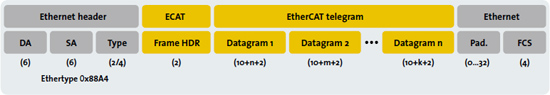
\includegraphics[width=0.8\textwidth]{EtherCAT_Technology_01_Protocol.jpg}
	\caption{EtherCAT frame structure \cite{protocol:ethercat}}
	\label{fig:ecat-frame}
\end{figure}

Datagrams include all information regarding data access which permit the master device to decide what data to access and when, meaning a fixed process data structure is not required.
Effectively, master devices can update variables with different cycle times, possibly relieving some processing power.
As an example, for a system that requires motion control, the motor drives can get their parameters updated with a 1ms period, while discrete Inputs/Outputs (I/Os) can be updated with a 20ms period (typical control applications).

Each slave contains a unique node address which is assigned during network configuration.
Because node addresses are static, they can be used to target the specific node, even if the underlying network topology changes.
In addition, slaves can also be addressed by their location on the network, but this is usually only used during network initialisation to check for topology changes.
This is done by comparing a configured list of node addresses and their location on the network with the discovered topology.

On system initialisation, multiple logical addresses can be configured on each node, allowing a single datagram to target multiple physical devices.
The cyclical exchange of process information uses logical addressing to execute the data transfers.

This type of addressing scheme also allows slave-to-slave communication.
There are two possibilities of achieving this:
\begin{enumerate}
	\item If the process structure is constant, sending data to another slave which is further downstream can be done in the same bus cycle;
	\item If the process is not constant or the network has a dynamic topology, slave-to-slave communication can go through the master device and, because of \emph{EtherCAT}'s performance, this is still faster than other traditional communication stacks (TCP/IP, UDP/IP, etc.).
\end{enumerate}

EtherCAT can also benefit from the modern system's \textbf Direct \textbf Memory \textbf Access (DMA) feature, which removes the necessity for a CPU to explicitly transfer data from physical RAM to a peripheral device.
This means that a master device application only needs to construct the EtherCAT frame and place it on a specific memory region, leaving the DMA controller to actually pass the data over to the Ethernet MAC controller, saving CPU for the actual data processing.


\subsubsection{Topology}

\emph{EtherCAT} supports a variety of network topologies like \emph{line}, \emph{tree}, \emph{star} or \emph{daisy-chain}.
When designing a certain network, multiple topologies can be combined into a hybrid topology network.
Many ESCs and Input/Output (I/O) modules already include ports to create network branches, which eliminates the need to use switches or any other type of infrastructure components.
Regardless, classical \emph{Ethernet} star topology can be used to implement an \emph{EtherCAT} network.

ESCs also include support for a ``Hot Connect'' feature which means existing nodes can be removed and new nodes can be added to the network during runtime.
The controllers can detect these changes in a very short time (typically less than 15$\mu$s), allowing a smooth state transition without interfering with the rest of the network.

There is also a big flexibility in terms of available cabling option, from inexpensive industrial \emph{Ethernet} cables to fiber optics, having the entire Ethernet wiring possibilities available for use.

EtherCAT gateways provide the means to incorporate other fieldbus networks as a subnetwork.
This allows a gradual changeover between fieldbuses by keeping network sections that may contain components which still do not support the EtherCAT interface.

Due to the fact that EtherCAT uses a 16-bit address length, up to $65535$ devices can exists in a single network segment, which makes scalability virtually unlimited.
This large device count removes the need to use bus extension methods, like traditional gateways, providing even the largest EtherCAT networks the best possible performance without delays.



\section{Summary} \label{sec:impl-summary}
This chapter focused almost exclusively on technical details of how the final solution was implemented.
Starting with the choice of hardware components, going through their assembly and then moving towards the complex and extensive software required to give the desired slave device all planned functionality.

Not only the good things have been explained but we have also expressed those we are aware could have been better implemented or designed.
Even though this project was developed during difficult times, especially from having been done entirely on a full-remote work basis, most of the things explained as weak spots were considered from the beginning.
Difficult times impose harder decisions and \emph{simplify} became the daily word of choice because, sometimes, \emph{less is much more}.
It's one thing to design simple systems, but it's a much harder thing to simplify complex systems and boil them down to their bare-bones.


\chapter{System architecture} \label{chap:sys-arch}

In this chapter we will present the architecture that has been defined for the demonstration system.
During the course of this project's development phase, its architecture was continuously adapted as difficulties and possibilities emerged with the advancements made.

The following descriptions will reflect the final state of the proposed demonstrator, after several incremental iterations.
In relevant portions of this work, some comparisons will be made with the initial planned architecture to, not only demonstrate the iterative development process adopted but also to highlight some key aspects that benefited from this type of approach.

We will begin this chapter with an analysis of the requirements we should meet in order for the demonstrator to have certain characteristics, then present a detailed explanation of the actual proposed architecture, including the chosen hardware and software, finishing with a brief and non-exhaustive description of some conceptual experiments that could be possibly demonstrated on the proposed platform.

\section{Requirements analysis} \label{sec:requirements}

% Simplicity
% Low cost
% Robust (SW & HW)
% Modularity
% Visually/Physically based
% Control:
% - DCS
% - Local & Remote control
% - Velocity & Position

When considering the development of any practical demonstrator, some generic requirements should be taken into consideration due to the scope of such products.
These become even more relevant when the demonstrator is designed for educational purposes, as this is one such scenario.

The following subsections will delve into the main requirements of our project, explaining why they are being considered a requirement, how they were dealt with during development phase, what difficulties were encountered to meet such need and in which manner each requirement influenced the final system.

\subsection{Simplicity}

The most important characteristic every demonstrator should own is simplicity.
No matter how complex or extensive the concept might be, good demonstrators are conceptually simple.
Designs that focus solely on the concept at hand and leave out superfluous functionality tend to be more effective at conveying the main message.
Having the ability to further explore the concept beyond the initial scope of the demonstrator by extending its capabilities could be an advantage, but only when the implications of doing so do not hurt the initial simplicity.

In order to design a good demonstrator, simplicity should be the main focus in the early stages of research and concept design.
Contemplating different approaches based on simple concepts is crucial to ensure the end result is focused on the correct concept.
It is also very important to not allow underlying characteristics or design choices to outweigh the core concept.

\subsection{Low-cost} \label{sec:low-cost}

Demonstrators whose purpose is to serve as a first contact mechanism under an educational directive should be as low-cost as possible.
Accidents, bad practices or the simple lack of necessary knowledge can lead students and first-timers to, unintentionally, damage educational equipment.

Students tend to learn more easily when left to their own experiments, learning by themselves how things work and how to operate them. % TODO Cite something
For this to be possible, educational equipment should not impose limitations on the user freedom and, to meet such goal, low-cost is generically the best option.
Students must be able to experiment and learn without having to constantly worry about possible damage to expensive equipment.

\subsection{Modularity}

In addition to what is described in \autoref{sec:low-cost}, designing a system based on well defined modules is always a good thing.
Modularity helps divide the most complex systems into several, easier to handle, parts.
This characteristic also helps reduce costs, especially when considering the integration of pre-made modules, instead of developing new ones.

When there is possibility to design a product that reuses components and modules available on the market, production, maintenance and repairs become simpler and cost-effective.
With this approach, a damaged physical module can simply be replaced and software modules become easier to work with.
When developing software modules, one needs to pay close attention to the planned boundaries of each module, making sure their functionality is entirely self-contained.
This way, if we wish to replace a physical module we can also simply swap the respective software module with a new one, targetted at the new physical module.

\subsection{DCS based architecture}

With our aim being the influence of network cycle time on control applications, it's imperative for us to use an architecture that resembles a DCS system.
It only makes sense to evaluate such influence on systems where it is applicable, meaning, we must replicate a real world case where the usage of an RTE might actually influence the system performance.
With this in mind, we decided to replicate the concept of a networked servo drive controlled from a centralized processing unit, with the ability for the control loop to be closed either locally on the servo drive (the current typical scenario) or remotely on the processing unit.


\section{Proposed implementation}
Following the proposed architecture, presented in the previous chapter, we will now explain the actual implementation we performed to achieve our goals.
This section briefly presents the overall idea and proposed system architecture without going into details about specific choices.
Those explanations will be presented in later sections, as we will delve deeper into the implementation details, including product and technology choices, both in terms of hardware and software.

\subsection{Master node}
The master node of our system will be implemented in a generic desktop PC through the usage of an industrial programming platform.
This will enable us to program the behaviour of the master node as well as provide the necessary communication libraries to implement a master node for different RTE networks.
We will take advantage of the fact that most industrial programming platforms allow us to determine the RTE network's update period.
This will enable us to perform tests using different network cycle times.

Two programs will be developed for the master node:
\begin{enumerate}
	\item one to act as a simple set-point generator, sending the velocity or position set-points to the slave device through the RTE network;
	\item a second one to act as the motion controller, where the same set-points are used internally in a control algorithm that receives the plant feedback value and sends the plant output value through the RTE network.
\end{enumerate}

This implementation will allow us to perform the two practical experiments described in \autoref{sec:experiments}, enabling us to compare performance values acquired in both cases.

\subsection{Slave node}
The proposed slave implementation will be based on an embedded computing platform.
The embedded platform will be extended using some specialised boards that will broaden the functionality of the slave device as a whole.
These extension will provide easier access to the GPIO pins, direct interface with a motor through a specialised DC motor control board and Real-Time Ethernet connection using a dedicated board capable of off-loading the real-time processing of network packets from the embedded computing platform.

Additionally, in order to create a connection with the real world, we'll be using a DC motor paired with an incremental encoder.
This will allow data to be collected from a real world source, giving a more organic feeling to the process of running experiments with this system.

In terms of software, a control application will be developed for the slave device computing platform in order to provide the following functionality on the slave device:
\begin{itemize}
	\item Handle the receiving and sending of cyclic data through the RTE network by interfacing with the driver of the dedicated RTE network connection board. Such data will include set-point and feedback values;
	\item Handle the plant feedback signals, converting them into internal variables.;
	\item Handle the motor output signal by interfacing with the dedicated DC motor control board;
	\item Acquire and export performance data relating to the control of the DC motor speed and/or position;
	\item Provide an internal control algorithm to locally control the motor's speed and/or position;
\end{itemize}

Such software will be implemented in modules, and a general overview of how they interconnect with each other can be seen in a block diagram format in \autoref{fig:sw-architecture}.
The block names represent the actual names used for the different modules that were implemented.

\begin{figure}[htp]
	\centering
	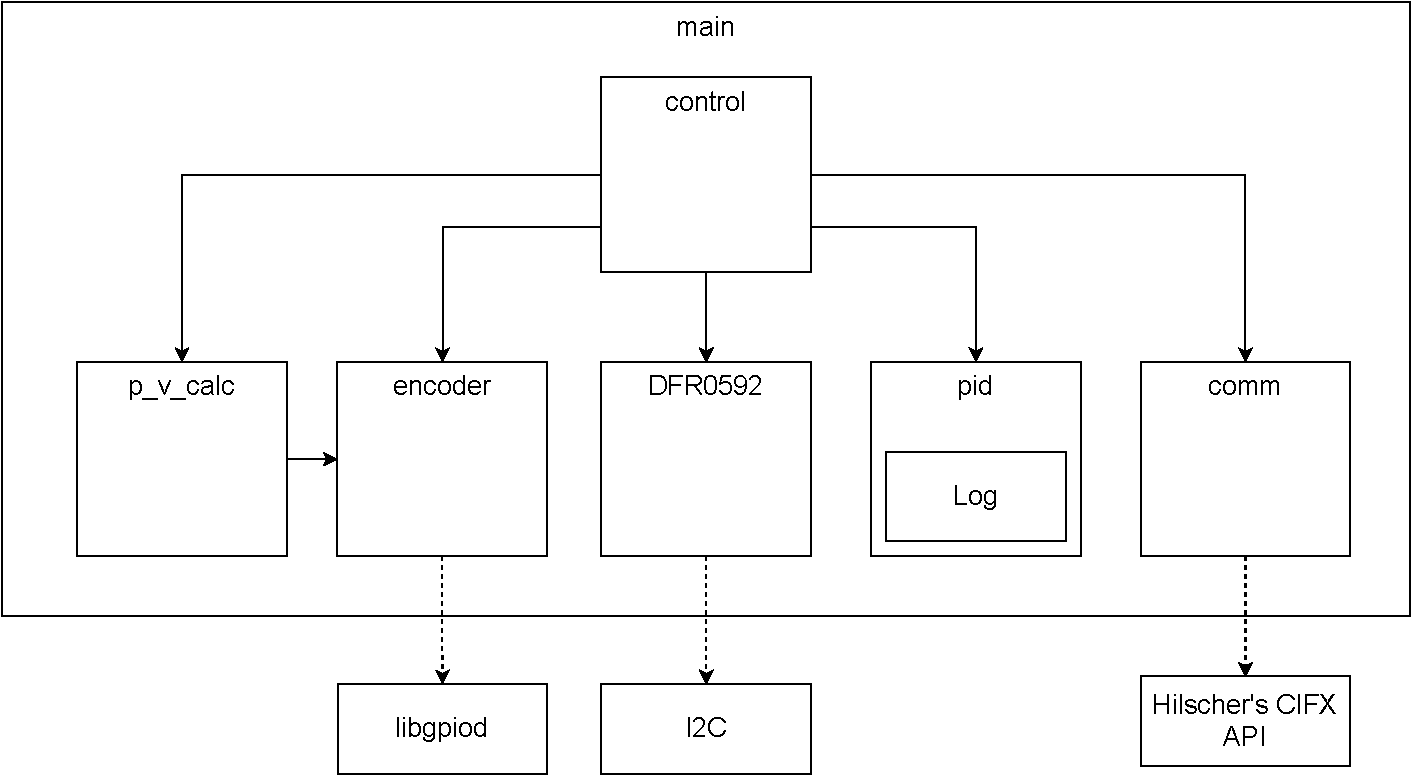
\includegraphics[width=0.8\linewidth]{sw-architecture.pdf}
	\caption{Slave device's software dependency graph}
	\label{fig:sw-architecture}
\end{figure}

The \verb|main| module will take care of initialising all data structures and sending the terminate commands when the user wishes to close the control application.
Configuration parameters can be passed as command-line arguments to the main module, which will be parsed and used during the run-time.
This module will serve as the entry point for the control application, where, after compilation, all modules will be integrated into a single executable.

The \verb|control| module will contain the function calls that determine the behaviour of the slave device during normal operation.
The run-time behaviour takes into consideration all parameters provided when launching the application.
It also takes care of moving data around between the other modules before calling functions that require some external data.
For example, the \verb|pid| module requires the set-point and plant feedback values, which are retrieved from the \verb|p_v_calc| module and \verb|comm| module, respectively.

The \verb|p_v_calc| module will be responsible for computing the motor velocity and position, based on an encoder counter.
Such counter is implemented on the \verb|encoder| module, which will convert the encoder signals onto a counter value.
In order to have access to the encoder signal, which will be connected to the GPIO header, we used the external library called \verb|libgpiod| to gain access to the GPIO pins.

The \verb|DFR0592| module is responsible for implementing functions to access and interface the DC motor control board.
All communication is done via I2C, which requires the usage of an external library.
In this particular implementation, we used the default Linux kernel I2C library.

The \verb|pid| module implements a discrete-time PID controller used for the local control of the motor's position or velocity.
Additionally, because all relevant data that describes the system performance is already contained in the PID data structure, we implemented the functionality of exporting such data on this module.

At last but not least, the \verb|comm| module will be responsible to make API calls to the RTE interface board driver, called \verb|CIFX|, in order to configure the RTE network and retrieve/send cyclic process data.
All the necessary steps to initialise, configure and manage the different RTE networks will already be implemented in the \verb|comm| module functions.


\section{Iterative process}

In the beginning of this project, while being to clouded with the idea of applying the concept to a robotic system, we explored several possibilities of creating a demonstrator based on a robotic arm.
The conceptual idea was to preprogram a path on the robotic arm that had to be followed when its actuators were commanded through a real-time network.
One could define a 2D path on a sheet of paper and the robotic arm would have to follow it with a pen, drawing the travelled path.
This way, the effects of network cycle time would be indirectly visible when comparing the preprogrammed path and the actual travelled path.

This concept had an interesting potential but soon enough we came across a not so obvious problem: from the user's point of view, when looking at a robotic arm system, the attention would almost certainly go towards what the robotic arm could do instead of focusing on what was happening in the background, especially in terms of communications and how they affected the control system.

After deciding this was not the way to go, we performed a retrospection exercise and analysed what was good about this first idea and why we had it in the first place.
The underlying concept that made us consider this approach is that robotic systems are characterized by one traversal aspect: movement control.
In fact, wanting to demonstrate the effects of network cycle time in a control application, controlling movement seems to best fulfil the purpose.
This type of control requires short cycle times and deterministic periodicity, making it very susceptible to the effects of network cycle time.
Additionally, it provides the demonstrator with a graspable connection to reality.

The second iteration on the base concept led us to an idea still based on movement control but with a simpler approach: two perforated discs attached to motors, facing each other, would have their movement controlled independently.
One of the discs would have a control loop closed locally on the field device and the other one would have it closed on the master controller node, traversing a real-time Ethernet network.
With both discs coupled with a single string of spaghetti pasta, any effects the real-time Ethernet network would introduce on the control system would make the two discs' movement desynchronise and, as such, it would manifest through the spaghetti string breaking.
We decided not to pursue this idea further because we expected, from the beginning, that the effects introduced by the communication network would have a small impact on performance and that, in this case, the spaghetti string would possibly have enough elasticity to withstand the small expected position slippages between the two discs.

Given the reason for discarding the second concept, we decided the best way to visualize such small differences would be to compare data points relative to the movement of both the locally and remote controlled runtimes.
In order to generate such data, virtually any type of physical movement can be utilized.
So, simplifying the second concept iteration into a third one, the idea was now to control the movement of a single disc.
The control itself can still be performed both locally on the field device or remotely on the master device, but not simultaneously.
This way, one can create a sequence of set-points and pass them to both types of control which, in turn, will generate data relative to the disc's movement.
One can then compare these data sets by creating graphs or using any other relevant methods.


\section{Conceptual experiments} \label{sec:experiments}

With the proposed architecture in mind, which was described in section \ref{sec:proposed-arch}, we have envisioned a generalized conceptual experiment to fulfil the main goal of demonstrating the effects of the network cycle time influence in control applications.
We have defined it in a generic way so that variations and extensions to the base idea can easily be developed.
This way the demonstrator does not focus on a single possible experiment but on a set of experiments that share the same foundation.

The first and most basic conceptual experiment we considered involves predefining a velocity curve over a certain amount of time and executing it using both available control modes: the local control and the remote control.
Each of these will generate a trace log of velocity points (in this case) measured during execution.

Naturally, the definition of the movement curve can be randomly generated or taken from any real-world example, whatever interests the user the most.
Independently of which control mode is going to be be executed, the predefined movement curve is to be stored in the master node by whatever means, either hard-coded into the control program or by using some form of data storage and interpretation.
Because the master node's software implementation will be left to the end-user's responsability, so will be the generation or interpretation of reference values from the predefined movement curve.
The only thing to be taken into account is that depending on which control mode is being used at a certain time, the slave device expects to receive different types of data: for local control the slave device expects to receive the control reference values (directly taken from the predefined movement curve) and for remote control it expects to receive the duty-cycle percentage to be applied to the motor (the actual 'output' value of the control loop).

As we aim to provide the means to export the recorded command and feedback values as a CSV file, we can now import them into any data processing software and perform relevant operations between the two traces.
The most simple comparison possible, and possibly the most effective, is to generate a graph that includes the two datasets simultaneously, which will create a visual representation of the system's performance in both control cases, making any differences in their behaviour quickly perceivable.




\section{Summary} \label{sec:impl-summary}
This chapter focused almost exclusively on technical details of how the final solution was implemented.
Starting with the choice of hardware components, going through their assembly and then moving towards the complex and extensive software required to give the desired slave device all planned functionality.

Not only the good things have been explained but we have also expressed those we are aware could have been better implemented or designed.
Even though this project was developed during difficult times, especially from having been done entirely on a full-remote work basis, most of the things explained as weak spots were considered from the beginning.
Difficult times impose harder decisions and \emph{simplify} became the daily word of choice because, sometimes, \emph{less is much more}.
It's one thing to design simple systems, but it's a much harder thing to simplify complex systems and boil them down to their bare-bones.


\chapter{Implementation} \label{chap:impl}

After having presented the proposed system architecture we will now move forward to describing how the project implementation was performed, starting with the evolution of the initial concept and then going through the hardware and software implementations.

This chapter will include very technical details especially during the software implementation explanaitions, so in order to have a good understanding of the implementation, basic knowledge of computer software is required.

\section{Concept development}

In the beginning of this project, while being to clouded with the idea of applying the concept to a robotic system, we explored several possibilities of creating a demonstrator based on a robotic arm.
The conceptual idea was to preprogram a path on the robotic arm that had to be followed when its actuators were commanded through a real-time network.
One could define a 2D path on a sheet of paper and the robotic arm would have to follow it with a pen, drawing the travelled path.
This way, the effects of network cycle time would be indirectly visible when comparing the preprogrammed path and the actual travelled path.

This concept had an interesting potential but soon enough we came across a not so obvious problem: from the user's point of view, when looking at a robotic arm system, the attention would almost certainly go towards what the robotic arm could do instead of focusing on what was happening in the background, especially in terms of communications and how they affected the control system.

After deciding this was not the way to go, we performed a retrospection exercise and analysed what was good about this first idea and why we had it in the first place.
The underlying concept that made us consider this approach is that robotic systems are characterised by one traversal aspect: movement control.
In fact, wanting to demonstrate the effects of network cycle time in a control application, controlling movement seems to best fulfil the purpose.
This type of control requires short cycle times and deterministic periodicity, making it very susceptible to the effects of network cycle time.
Additionally, it provides the demonstrator with a graspable connection to reality.

The second iteration on the base concept led us to an idea still based on movement control but with a simpler approach: two perforated discs attached to motors, facing each other, would have their movement controlled independently.
One of the discs would have a control loop closed locally on the field device and the other one would have it closed on the master controller node, traversing a real-time Ethernet network.
With both discs coupled with a single string of spaghetti pasta, any effects the real-time Ethernet network would introduce on the control system would make the two discs' movement desynchronise and, as such, it would manifest through the spaghetti string breaking.
We decided not to pursue this idea further because we expected, from the beginning, that the effects introduced by the communication network would have a small impact on performance and that, in this case, the spaghetti string would possibly have enough elasticity to withstand the small expected position slippages between the two discs.

Given the reason for discarding the second concept, we decided the best way to visualise such small differences would be to compare data points relative to the movement of both the locally and remote controlled run times.
In order to generate such data, virtually any type of physical movement can be utilised.
So, simplifying the second concept iteration into a third one, the idea was now to control the movement of a single disc.
The control itself can still be performed both locally on the field device or remotely on the master device, but not simultaneously.
This way, one can create a sequence of set-points and pass them to both types of control which, in turn, will generate data relative to the disc's movement.
One can then compare these data sets by creating graphs or using any other relevant methods.


\section{Parts choice} \label{sec:parts_choice}
During the development phase of the project, some hardware components needed to be chosen in order for us to be able to actually develop a prototype system.
With components ranging from a full computing platform to a simple electrical connection board, we will briefly introduce the necessary hardware as well as provide an explanation about the logic utilized during the decision period.

% Parts choice
% `- Motor & Encoder
% `- DFR0592
% `- Raspberry Pi
% `- netHAT 52-RTE
% `- screw terminal add-on

\subsection{Raspberry Pi 4} \label{subsec:rpi4}
The Raspberry Pi 4 is a single board computer (SBC) and comes equipped with the Broadcom's BCM2711, a quad-core Cortex-A72 64-bit ARM processor clocked at 1.5GHz \cite{technology:rpi4-specs}.
At the time of writing, versions were available with 2GB, 4GB and 8GB of LPDDR4 SD-RAM \footnote{Low-Power Double Data Rate Synchronous Dynamic Random-Access Memory} clocked at 3200MHz.

This version of the Raspberry Pi series is the first to be equipped with a true-Gigabit Ethernet controller connected to the PCIe bus, while earlier versions used a USB attached one, meaning latency and throughput were not as good and especially less constant.

As our designed slave device is intended to be used in headless mode, meaning no monitor output and no keyboard nor mouse will be used, we picked the version with 2GB of RAM.
As no graphical interface needs to be created, memory usage will be very reduced and, as such, 2GB are plenty of memory for our needs.

The Raspberry Pi 4 incorporates a micro-SD card slot to be used as an embedded hard disk, so we have also included a small 16GB micro-SD card to serve as such.
Linux is a very small operating system and a fresh install of Raspberry Pi OS Lite occupies about 1.4GB, meaning the 16GB of space are more than sufficient for our needs.

% Conclusion
During the development phase we have considered the Raspberry Pi 4 to be the most appropriate solution for the project's slave computing platform.
Its features and characteristics seemed to fit the requirements well, so we locked our choice for this equipment.

\subsection{Motor \& encoder}
% `- DC motor
% `- Encoder
% `- Why not standard servo motor + drive
In order to provide our system with the physical connection with the world we aim for, we have chosen a small 6V brushed DC motor with an embedded 30:1 gearbox \cite{product:pololu-micrometal-gearmotor}.
This motor provides an extended shaft on the back of the motor so that a magnetic encoder kit can be attached to it.

Pololu \cite{brand:pololu}, which is the maker of our chosen motor, separately provides the magnetic quadrature encoder kit, compatible with such motor, with a resolution of 12 pulses per revolution (PPR) in quadrature mode.
A preview picture of the motor + encoder kit can be seen in \autoref{fig:encoder_motor}.
The encoder provides quadrature signals A and B at the same voltage as its power supply.
It is rated to be powered between 2.7V and 18V, allowing it to used for a wide variety of applications.

\begin{figure}[htp]
	\centering
	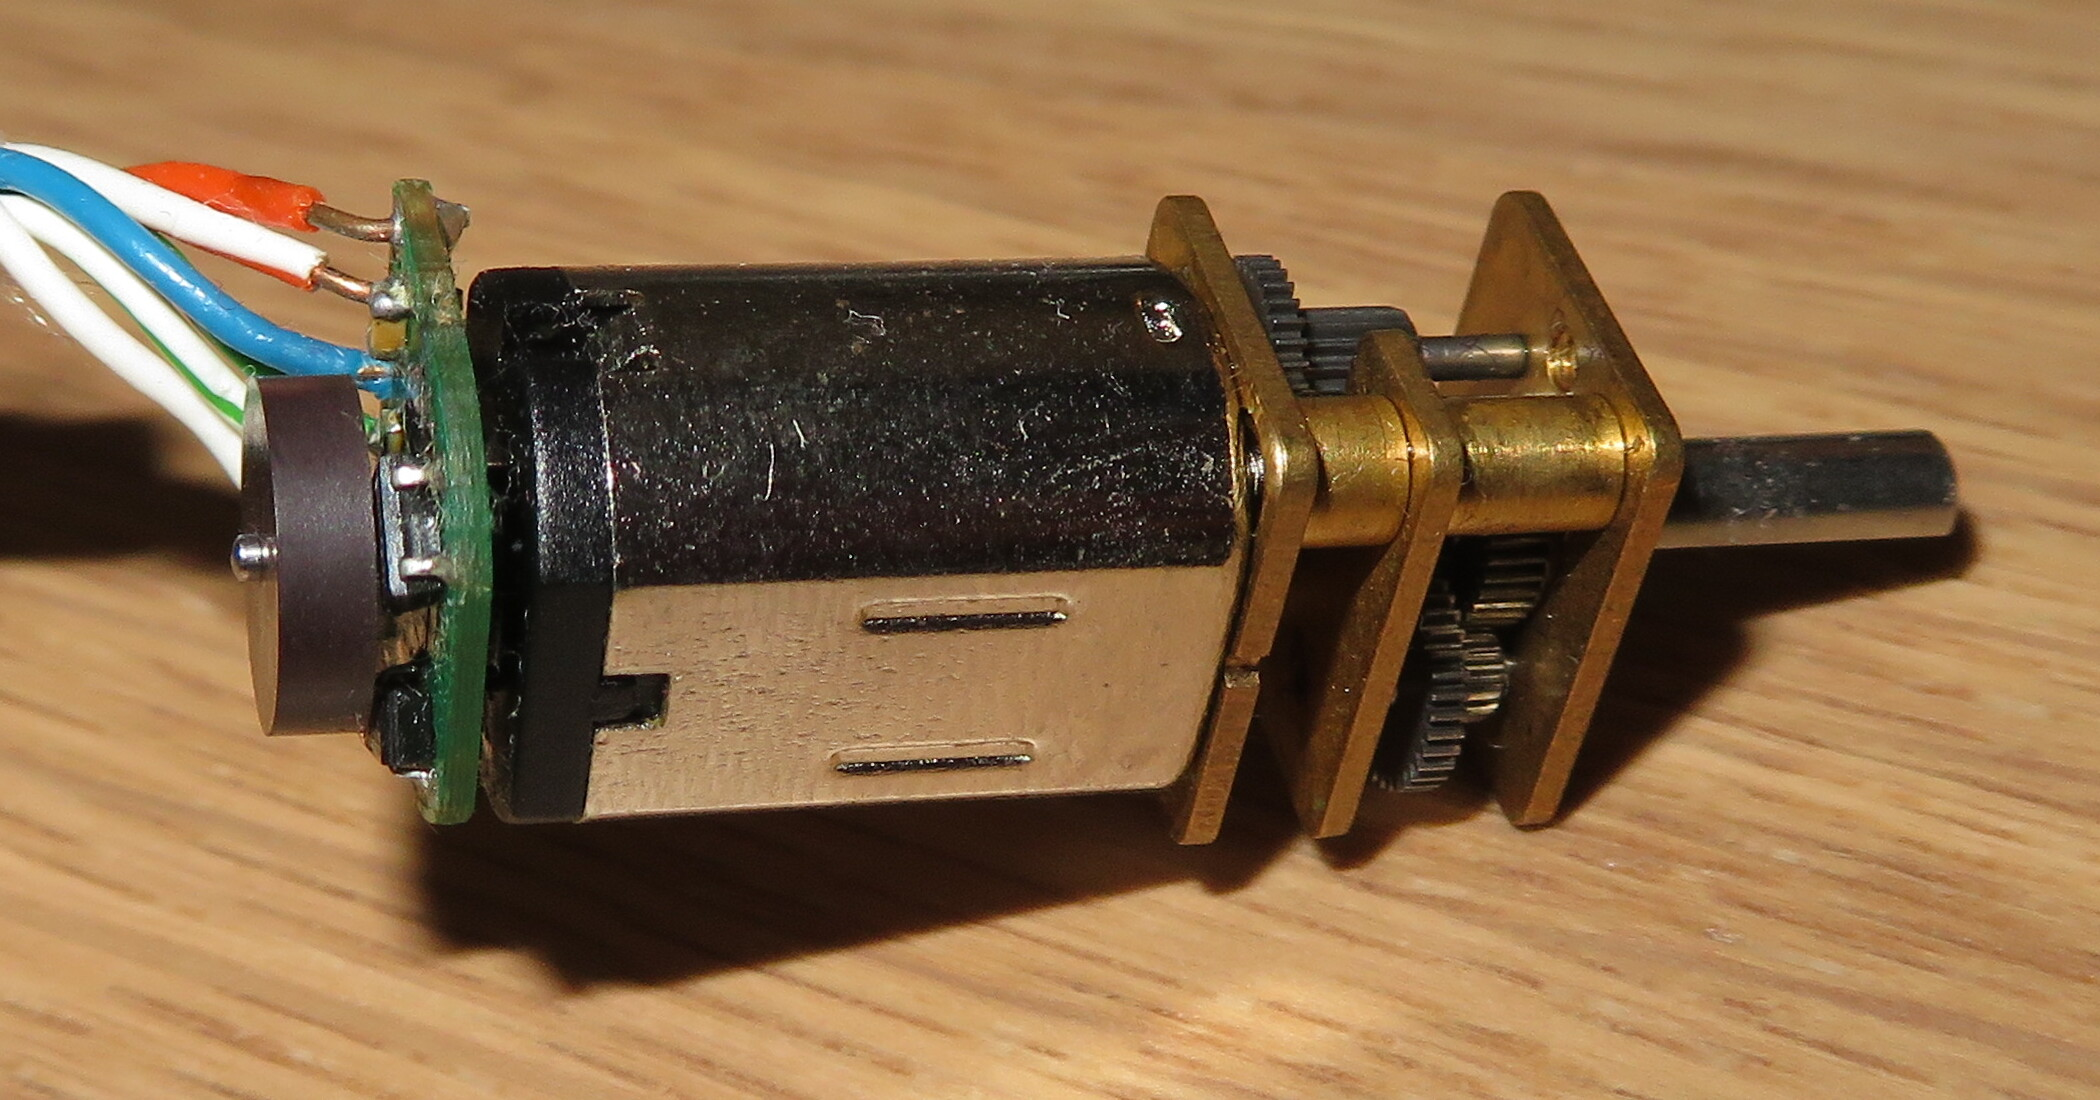
\includegraphics[width=0.8\linewidth]{encoder_motor.JPG}
	\caption{Detail of the DC gearmotor and attached magnetic encoder}
	\label{fig:encoder_motor}
\end{figure}

Incremental quadrature encoders are very commonly used in the industry, mostly due to their simplicity and modest prices, when compared with absolute encoders.
The encoder provides two electrical signals (A and B) which change their values according to the motor angular displacement.
The two electrical signals are said to be in quadrature because they have a phase shift of 90\textdegree{} between them, meaning they will never change state simultaneously.
While rotating, the A and B signals will continuously change their state between 0 and 1, as seen in \autoref{fig:quad-encoder}.
The direction of rotation can be determined by evaluating the relative phase shift between those signals.
If we take signal A as reference and determine that signal B has a +90\textdegree{} phase shift relative to A while rotation clockwise, then a counter-clockwise rotation will generate a B signal with a -90\textdegree{} phase shift relative to A.

\begin{figure}[htp]
	\centering
	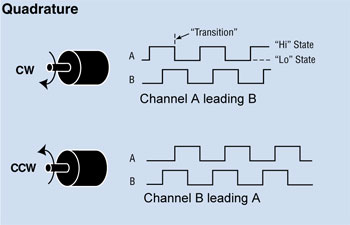
\includegraphics[width=0.8\linewidth]{quad-encoder.jpg}
	\caption{Working principle of an incremental quadrature encoder (Adapted from \cite{technology:quad-encoder})}
	\label{fig:quad-encoder}
\end{figure}

An encoder that is said to have a resolution of 12PPR in quadrature mode means that each quadrature signal (A and B) will generate 3 pulses per revolution.
Therefore, we can catch 6 state changes on each of those signals, providing us a total of 12 pulses per revolution, between the two signals.
A example of such counting method can be seen in \autoref{fig:quad-encoder-2}.

\begin{figure}[htp]
	\centering
	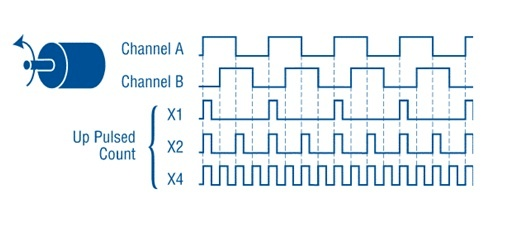
\includegraphics[width=0.8\linewidth]{quad-encoder-2.jpg}
	\caption{Detail of the quadrature count mode (Adapted from \cite{technology:quad-encoder})}
	\label{fig:quad-encoder-2}
\end{figure}

The power supply range allows it to be directly connected to the Raspberry Pi GPIO pins, which only works with 3.3V.
This is an advantage that most encoders available on the market do not offer, as they are usually rated for standard industrial power supplies such as 5V, 12V and 24V, which are the most common.
Additionally, the DC motor is rated for a 6V-9V supply.
As the DFR0592 board (see \autoref{subsec:dfr0592}) can provide between 7V and 12V on the motor outputs, depending on the actual power supply used, the entire kit contains components fully compatible between themselves.

Because the DC motor includes a 30:1 reduction gearbox, the resulting encoder precision is multiplied by that ratio, giving the output a virtual encoder resolution of 360PPR.
For a proof-of-concept system, this is enough precision for position control, providing a maximum error of 1 degree.
This DC motor has a theoretical maximum velocity on the output shaft of 1100RPM.
This means that encoder pulses will be generated, while at full speed, at a rate of $396000$ pulses per minute, or $6600$ per second.
For velocity control, the maximum amount of pulses generated per second is not too high so the Raspberry Pi should be perfectly capable of not missing pulses.

This solution allow us to maintain a low budget for the project and is the main reason we have not chosen to use a standard servo motor paired with a servo drive, although we have considered it.
These two parts would cost more than 400\texteuro, as that was the lowest price we could find on the national market.
Instead, the above mentioned motor and encoder kit summed up to about 30\texteuro, taxes included.

\subsection{DFRobot's DFR0592} \label{subsec:dfr0592}
% Intro
The DFR0592 board from DFRobot is an all-in-one DC motor control board with integrated quadrature encoder interface, PWM generation, an H-bridge for direct motor interface and an integrated micro-controller (an STM32 chip) that takes care of calculating the motor speed in revolutions per minute (RPM).
This board is an add-on HAT for the Raspberry Pi that uses the Inter Integrated Communication (I\textsuperscript{2}C or I2C) protocol to exchange information with the Raspberry Pi.
A preview image of this board can be seen in \autoref{fig:dfr0592-2}.

\begin{figure}[htp]
	\centering
	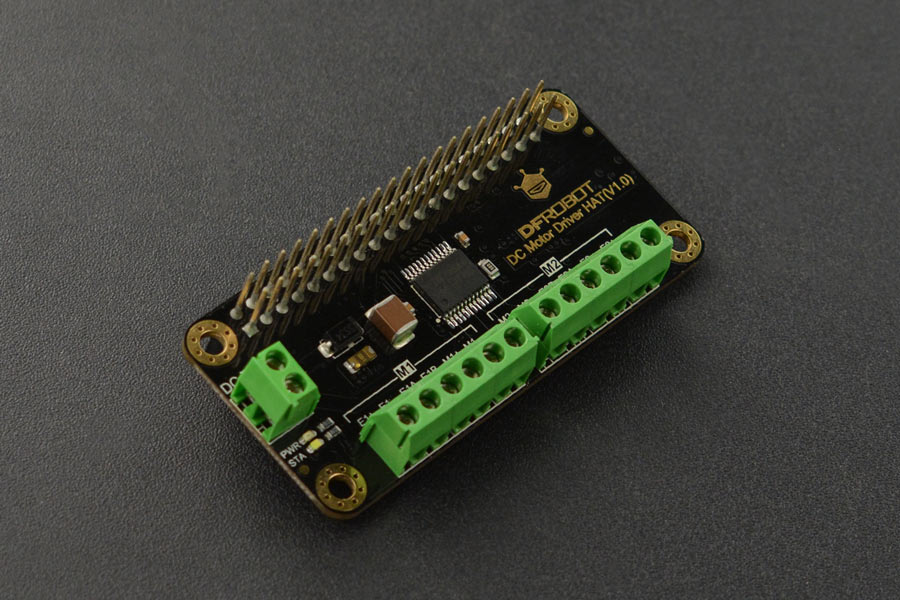
\includegraphics[width=0.8\linewidth]{DFR0592.jpg}
	\caption{DFRobot's DFR0592 board (adapted from \cite{hdw:dfr0592})}
	\label{fig:dfr0592-2}
\end{figure}

% Motor control
This control board takes some configuration values from the Raspberry Pi, such as the motor type (DC or stepper motor), PWM frequency, encoder ratio and others.
For the actual motor control, two values are needed: the direction of rotation (clockwise or counter-clockwise, obviously the motor terminals need to be assigned correctly) and the PWM duty cycle to be used (which is equivalent to saying the percentage of maximum power to apply).

% Conclusions
At first, this board seemed the best fit for the project, but after some preliminary testing, we found that the velocity calculation algorithm was only updating the feedback value every 100ms, which is to great of a period to use for movement control.
It could be acceptable for simple velocity control, but it would also limit the remote operation of the slave device by making it to slow for the desired application.

\subsection{Hilscher's netHAT 52-RTE}
As explained in the previous chapter, our project involves the development of a custom EtherCAT slave device.
For this, we need a specialized hardware interface called an EtherCAT Slave Controller (ESC).
As we have chosen to use a Raspberry Pi as our computing platform, we now require an appropriate ESC HAT board.
We will be using the Hilscher's netHAT 52-RTE \cite{hdw:nethat-52rte} board mostly because FEUP / DEEC had a set of them available for immediate use, so we did not have the necessity to order any for the development of the project.
A preview picture of this board can be seen in \autoref{fig:nethat-52-rte-2}.

\begin{figure}[htp]
	\centering
	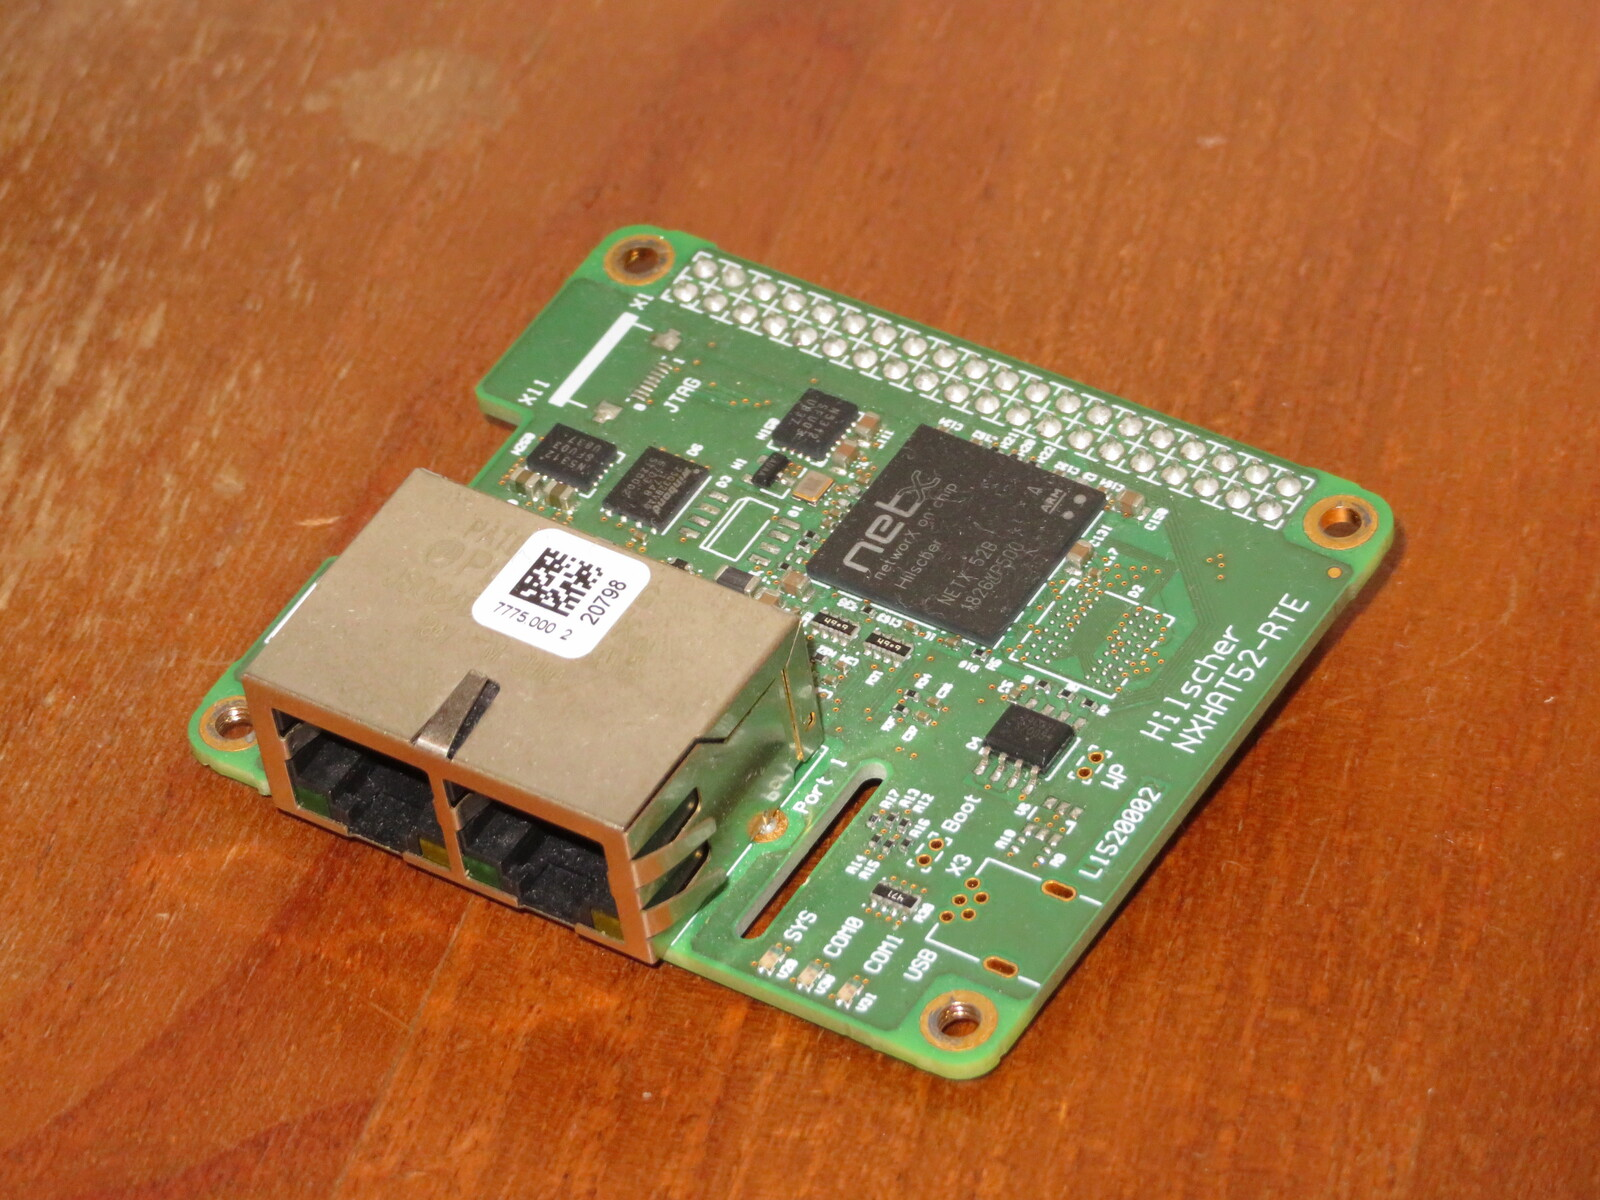
\includegraphics[width=0.8\textwidth]{nethat_52rte.JPG}
	\caption{Hilscher's netHAT 52-RTE board}
	\label{fig:nethat-52-rte-2}
\end{figure}

% HDW specs
The netHAT 52-RTE board has two Ethernet ports so that most of the supported EtherCAT network topologies can be implemented without the need for additional network hardware.
This board uses the Serial Peripheral Interface 0 (SPI0) of the Raspberry Pi for communication and uses a mailbox system to deliver messages to the control program.
The ESC chip allows cyclic synchronisation of 32 bytes of input and 32 bytes of output data.
Considering our project will only require a few bytes for each data type, there is plenty of room to do so.

% SW stuff
This board provides an API library for the C language so developers can program the desired slave device behaviour.
The documentation manuals (\cite{nethat:cifx_api_docs} and \cite{nethat:ethercat_api_docs}) provide useful and insightful information on how this ESC board works and how to use it properly.
These were the main references used during the development of the slave device software, especially during the development of the helper function that interact with the netHAT API library.

\subsection{Screw terminal GPIO interface}
This piece of hardware was necessary in order to connect the above mentioned motor encoder to the Raspberry Pi.
The previously referred stack boards do not provide any external access to the Raspberry Pi's GPIO pins and the Hilscher's netHAT 52-RTE board forces its placement on the top of the stack without providing a pass-through connector.

This specific model has been chosen for its simplicity, reduced cost and ease of use, as connecting the encoder wires is very easy and it provides a stable electrical connection due to the usage of screw terminals.
Unfortunately this model has been discontinued but any generic GPIO expansion board should do the job of exporting the electrical connection needed to interface with the encoder.


\subsection{Hardware} \label{sec:proposed-hardware}

While keeping a careful consideration of characteristics between options and maintaining the requirements in focus, hardware parts were chosen to build each section of the demonstrator.

\subsubsection{Master node}

Taking into account the two operation modes the demonstrator should have, we extrapolated that the master node must be able to perform numeric calculations and serve as an EtherCAT master device.
As the EtherCAT master implementation can be done using a generic Ethernet MAC interface card (refer to \ref{subsubsec:master_devices} for an explanation), everything the master node requires in term of hardware is a computational platform (computer, microcontroller, etc.) with access to a generic Ethernet MAC interface card.

As of today, most education facilities provide students with access to desktop computers.
For many years now, motherboard vendors have integrated Ethernet MAC interface cards into the motherboards themselves, as it has become the \emph{de facto} standard for Internet connectivity in desktop computers.

As such, we decided to implement the master device in a desktop computer in order to minimize costs and leverage the computational power modern computer systems possess.

\subsubsection{Slave node} \label{subsubsec:slave_hdw}

On the other hand, the slave node's hardware was harder to choose.
In order to implement the desired EtherCAT slave (see \ref{subsubsec:slave_devices}), one must be aware when choosing a computational platform to check the availability of a fitting ESC board and, simultaneously, the support for motor and encoder interfaces.

After some research, two options presented themselves as possible platforms for the slave device: an Arduino UNO or a Raspberry Pi.
ESC boards exist for both these platforms, as well as good support in terms of "shield boards" for motor interfaces.
In the end, we decided to go with a solution based on a Raspberry Pi, as it provides a more robust and versatile computing platform, especially considering the local control configuration, where position/velocity control algorithms will need to be executed on this platform.

The ESC board chosen for the Raspberry Pi was the Hilscher's \emph{netHAT 52-RTE} (see \url{www.netiot.com/interface/nethat}).
This board supports communication with three real-time Ethernet protocols (PROFINET, EtherNet/IP or EtherCAT), chosen with a simple firmware loading procedure.
It complies with the Hardware Attached on Top (HAT) specification for the Raspberry Pi (see \url{www.github.com/raspberrypi/hats}) and uses the \emph{SPI0} interface to communicate with it.
The board also includes the respective Electronic Data Sheet (EDS) files to be imported by the EtherCAT master, used to identify the characteristics and functionality of slaves implemented using this setup.

% Motor choice

With the intention to relieve the Raspberry Pi from having to generate the PWM signal to drive the motor, we included the DFRobot's DFR0592 board onto the design.
This board also complies with the HAT specification and communicates with the Raspberry Pi via the Inter-Integrated Circuit (I\textsuperscript{2}C or I2C) interface.
It provides interface with two DC motors and two incremental encoders, all managed by an STMicroelectronics's STM32 chip.
The motor interface also includes the necessary DC-motor driver chip, allowing direct connection of the motor's terminals and power supply to the board itself.

Initially we planed on using this board's incremental encoder interface to also relieve the Raspberry Pi from such task but, as our preliminary tests concluded, it only exports the Revolutions Per Minute (RPM) value extrapolated from the encoder's pulse count and not the pulse count itself.
Furthermore, the RPM value is only updated once every 100ms, which is to large of a period for motion control.

\begin{figure}[htp]
	\centering
	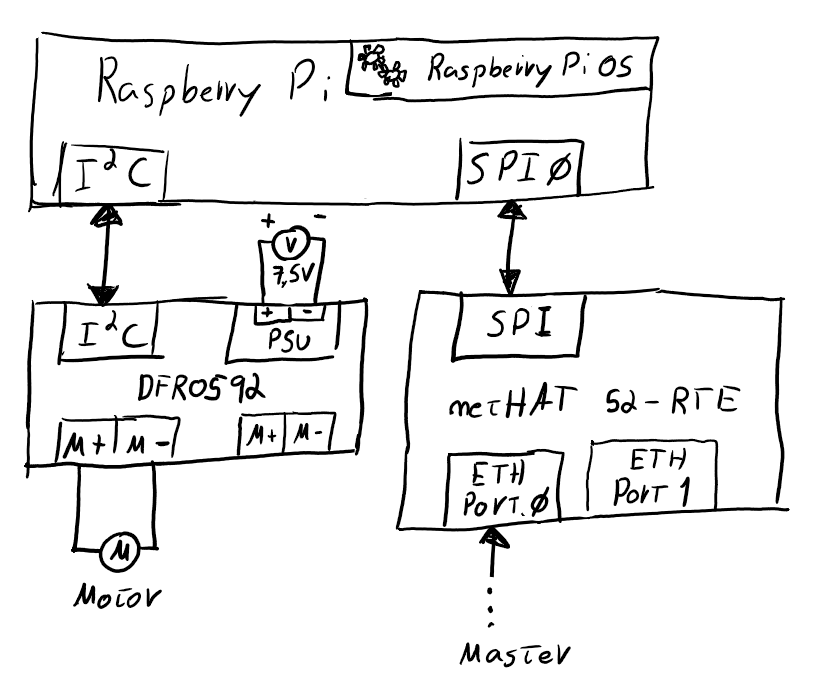
\includegraphics[width=1\textwidth]{slave_architecture.png}
	\caption{Graphical representation of the remote control scheme}
	\label{fig:slave_architecture}
\end{figure}\footnote{placeholder image}


\subsection{Software} \label{sec:proposed-software}

As can be expected, recent digital computing platforms require software to perform the necessary tasks.
As such, both the master node (computer) and the slave device (Raspberry Pi) will each require an Operating System (OS) to manage the execution of tasks.
The Raspberry Pi has a dedicated Linux OS called \emph{Raspberry Pi OS}, which is a fork from Debian (see \url{https://www.raspberrypi.org/software/}.
We will be using the Lite version of this OS for the Raspberry Pi as it is the easiest to setup and the most tested and stable OS for this platform.
Regarding the master node computer we will be using Microsoft's Windows 10 as the chosen OS, not only because most computers come pre-installed with it, but also because it is one of the few supported OSes by the CODESYS development application \cite{ide:codesys}, presented below.

\subsubsection{Master node software}

In order for us to create a control application on a generic computer, an appropriate software platform must be chosen.
Because we are working with industrial technology, a proper industrial control and automation software should be used.

CODESYS is a generic platform to develop industrial control and automation applications based on the IEC 61131-3 standard.
It includes support for hardware from multiple vendors as well as the ability to create a Software PLC (SoftPLC) from any generic computer hardware.
This platform makes the software editor available to use for free and allows control applications to run for two hours in demonstration/testing mode, uninterrupted.
This is a great option for development and testing purposes as only the final product with uninterrupted execution requirements for unknown periods of time will require a license to be purchased.
Additionally, CODESYS natively supports the most common industrial communication networks, including EtherCAT, meaning one can develop a device with communication capabilities with one or more of these networks.

With all this, we will use the CODESYS platform to create a SoftPLC to act as an EtherCAT master device for or demonstrator.
As we are looking forward to develop a proof-of-concept system, we don't require application runtimes larger than two hours.

Because we want to involve the end-user into the process of setting-up and running the experiments by themselves, we decided to leave the implementation of the master node's software to be dealt with by the end-user.
By doing such, we will also be indirectly expanding the set of conceptual experiments the demonstrator can handle by allowing anyone to implement their own ideas, as the slave device will always work the same way.

\subsubsection{Slave node software}

After having chosen the Hilscher's ESC HAT for the Raspberry Pi (see \ref{subsubsec:slave_hdw}), which will be running a Linux distribution, and decided to use the CODESYS platform for the master, we initially planned to also use CODESYS to program the slave device.
Although its editor is only designed to work under Windows, the SoftPLC runtime can run under Linux, with a version specifically targeting the Raspberry Pi platform.
Unfortunately, CODESYS doesn't support developing programs for EtherCAT slave devices, specifically, as these are usually programmed by manufacturers themselves and not by a system integrator or end-user.

Additionally, Hilscher only provides a library and accompanying API definitions for the C programming language, meaning at least the software module that needs to interact directly with the ESC will need to be programmed in C language.
As this is the most widely used programming language in the Linux universe, if during development we conclude we require some library to provide us with some advanced functionality, the probability of existing one for the C language is much higher than with less widespread languages.
As such, this is going to be our preferred programming language for implementing the EtherCAT's slave software running on the Raspberry Pi.




\section{Summary} \label{sec:impl-summary}
This chapter focused almost exclusively on technical details of how the final solution was implemented.
Starting with the choice of hardware components, going through their assembly and then moving towards the complex and extensive software required to give the desired slave device all planned functionality.

Not only the good things have been explained but we have also expressed those we are aware could have been better implemented or designed.
Even though this project was developed during difficult times, especially from having been done entirely on a full-remote work basis, most of the things explained as weak spots were considered from the beginning.
Difficult times impose harder decisions and \emph{simplify} became the daily word of choice because, sometimes, \emph{less is much more}.
It's one thing to design simple systems, but it's a much harder thing to simplify complex systems and boil them down to their bare-bones.


\chapter{Proposal evaluation} \label{chap:eval}
In this chapter we will present a practical experiment we conducted and present the resulting data.
This experiment will serve as a foundation for the evaluation of the designed system, by allowing us to verify which goals have been met and to which extent the project can be considered successful.

After having done so, we will also explain the limitations and design choices that were known to limit the outcome, up to a certain degree.
These limitations were mainly due to design choices and all of them were pondered from the beggining.
Certain features or components were only left out or replaced by simpler versions after making sure they would only reduce user friendliness or not include some advanced functionality to the system, not part of the scope of the original proposition.
As the result of this project is intended to be a proof of concept, aditional features and user friendliness was only an optional objetive.

\section{Conceptual experiments} \label{sec:experiments}

With the proposed architecture in mind, which was described in section \ref{sec:proposed-arch}, we have envisioned a generalized conceptual experiment to fulfil the main goal of demonstrating the effects of the network cycle time influence in control applications.
We have defined it in a generic way so that variations and extensions to the base idea can easily be developed.
This way the demonstrator does not focus on a single possible experiment but on a set of experiments that share the same foundation.

The first and most basic conceptual experiment we considered involves predefining a velocity curve over a certain amount of time and executing it using both available control modes: the local control and the remote control.
Each of these will generate a trace log of velocity points (in this case) measured during execution.

Naturally, the definition of the movement curve can be randomly generated or taken from any real-world example, whatever interests the user the most.
Independently of which control mode is going to be be executed, the predefined movement curve is to be stored in the master node by whatever means, either hard-coded into the control program or by using some form of data storage and interpretation.
Because the master node's software implementation will be left to the end-user's responsability, so will be the generation or interpretation of reference values from the predefined movement curve.
The only thing to be taken into account is that depending on which control mode is being used at a certain time, the slave device expects to receive different types of data: for local control the slave device expects to receive the control reference values (directly taken from the predefined movement curve) and for remote control it expects to receive the duty-cycle percentage to be applied to the motor (the actual 'output' value of the control loop).

As we aim to provide the means to export the recorded command and feedback values as a CSV file, we can now import them into any data processing software and perform relevant operations between the two traces.
The most simple comparison possible, and possibly the most effective, is to generate a graph that includes the two datasets simultaneously, which will create a visual representation of the system's performance in both control cases, making any differences in their behaviour quickly perceivable.




\section{Limitations} \label{sec:limitations}




\chapter{Conclusions} \label{chap:concl}

\section{Experimental results} \label{sec:exp-results}




\section{Goals met} \label{sec:goals-met}
After analysing the experimental data gathered in the previous chapter and retrospectively looking back at the original objectives of this project, we can only conclude that all main objectives have successfully been achieved with the terminus of the project.

Some advanced functionality we had planned at the beginning ended up not being implemented, especially improvements addressing mostly user friendliness and ease of use on the software front.
But, as explained in a previous chapter, a proof-of-concept system is not a final product.
All the essential features and desirable characteristics have been implemented, per the project requirements.

The experimental results confirm the validity of the system proposed in this document and provide a good indication that future works based on the presented concept are likely to produce positive results.
Eventually, more advanced designs could be able to port the concept to other scientific domains other than automation engineering.

After taking a step back and taking a perspective look towards the project as a whole, the difficulties that we overcame, the results we gathered and the goals we had established in the beginning, one conclusion I have definitely reached is that the initial concept ideas would have been to complex for the task at hand.
The results obtained in such cases would have been influenced by many uncontrollable factors and would probably not reflect as much the concept we set out to explore: the network cycle time influence in control applications using Real-Time Ethernet networks.

Although simple, the developed system and concept have been able to produce results with minimum external influence.
As said before, most times implementing and designing less can mean much more, and the results are proof of that.
A barebones Distributed Control System has allowed us to explore the influence of the network cycle time on control systems.

As explained in the introduction sections, we aim at providing a solid foundation on which more advanced concepts and systems ban be built upon.
We have followed and fulfilled all requirements that have been presented alongside the concept and we can only hope that such requirements have been correctly evaluated, because now only time will tell if the proposed system is solid, robust and flexible enough to be built upon.


\section{Future work} \label{sec:future-work}





%% comment next 2 commands if numbered appendices are not used
%\appendix
%\chapter{Loren Ipsum} \label{ap1:loren}

Depois das conclusões e antes das referências bibliográficas,
apresenta-se neste anexo numerado o texto usado para preencher a
dissertação.

\section{O que é o \emph{Loren Ipsum}?}

\emph{\textbf{Lorem Ipsum}} is simply dummy text of the printing and
typesetting industry. Lorem Ipsum has been the industry's standard
dummy text ever since the 1500s, when an unknown printer took a galley
of type and scrambled it to make a type specimen book. It has survived
not only five centuries, but also the leap into electronic
typesetting, remaining essentially unchanged. It was popularised in
the 1960s with the release of Letraset sheets containing Lorem Ipsum
passages, and more recently with desktop publishing software like
Aldus PageMaker including versions of Lorem Ipsum. 

\section{De onde Vem o Loren?}

Contrary to popular belief, Lorem Ipsum is not simply random text. It
has roots in a piece of classical Latin literature from 45 BC, making
it over 2000 years old. Richard McClintock, a Latin professor at
Hampden-Sydney College in Virginia, looked up one of the more obscure
Latin words, consectetur, from a Lorem Ipsum passage, and going
through the cites of the word in classical literature, discovered the
undoubtable source. Lorem Ipsum comes from sections 1.10.32 and
1.10.33 of ``de Finibus Bonorum et Malorum'' (The Extremes of Good and
Evil) by Cicero, written in 45 BC. This book is a treatise on the
theory of ethics, very popular during the Renaissance. The first line
of Lorem Ipsum, ``Lorem ipsum dolor sit amet\ldots'', comes from a line in
section 1.10.32.

The standard chunk of Lorem Ipsum used since the 1500s is reproduced
below for those interested. Sections 1.10.32 and 1.10.33 from ``de
Finibus Bonorum et Malorum'' by Cicero are also reproduced in their
exact original form, accompanied by English versions from the 1914
translation by H. Rackham.

\section{Porque se usa o Loren?}

It is a long established fact that a reader will be distracted by the
readable content of a page when looking at its layout. The point of
using Lorem Ipsum is that it has a more-or-less normal distribution of
letters, as opposed to using ``Content here, content here'', making it
look like readable English. Many desktop publishing packages and web
page editors now use Lorem Ipsum as their default model text, and a
search for ``lorem ipsum'' will uncover many web sites still in their
infancy. Various versions have evolved over the years, sometimes by
accident, sometimes on purpose (injected humour and the like). 

\section{Onde se Podem Encontrar Exemplos?}

There are many variations of passages of Lorem Ipsum available, but
the majority have suffered alteration in some form, by injected
humour, or randomised words which don't look even slightly
believable. If you are going to use a passage of Lorem Ipsum, you need
to be sure there isn't anything embarrassing hidden in the middle of
text. All the Lorem Ipsum generators on the Internet tend to repeat
predefined chunks as necessary, making this the first true generator
on the Internet. It uses a dictionary of over 200 Latin words,
combined with a handful of model sentence structures, to generate
Lorem Ipsum which looks reasonable. The generated Lorem Ipsum is
therefore always free from repetition, injected humour, or
non-characteristic words etc. 


%%----------------------------------------
%% Final materials
%%----------------------------------------

%% Bibliography
%% Comment the next command if BibTeX file not used
%% bibliography is in ``myrefs.bib''
\PrintBib{bibliography}

%% Index
%% Uncomment next command if index is required
%% don't forget to run ``makeindex thesis'' command
%\PrintIndex

\end{document}
